Obvious is a set of interfaces and extension classes for wrapping
around existing information visualization toolkits.  It generalizes
and extend the standard architecture as defined in the Information
Visualization reference model to try to abstract all the existing
implementations.  In this section, we list all of the existing
toolkits and explain what is common and how they differ.  In the
second section, we describe the most common standardization processes
for software systems.

\subsection{Visualization Toolkits}

Mostly all the existing information visualization toolkits follow the
InfoVis reference model initially specified by Ed Chi and refined by
Card, Mackinlay and Shneiderman~\cite{ChiRefModel,ReadingsIV}.  The
model defines three stages: Data Table, Visual Structure and View
(Figure~\ref{fig:refmodel}).  One of its main value is that is
explicitly represents the interaction, in contrast with older
visualization models.
Several articles have described the concrete design of an information
visualization toolkit.  We report here on the common and the
specific parts.

The InfoVis Toolkit~\cite{InfoVis} is based on an \emph{in-memory
  database manager} where data is organized in columns --- contrary to
most relational databases --- to improve the memory footprint and
allow adding new attributes that are needed to manage the interaction
(e.g. selection or filtering) and to hold attributes computed on
demand.  The main challenge being the support of interactive
performance for rendering and dynamic queries with a small memory
footprint.  The visual structure is managed using a \emph{monolithic}
architecture~\cite{Polylithic}: each visualization technique is
implemented as a specific class (e.g. ScatterplotVisualization,
ParallelCoordinatesVisualization, TreeVisualization) that performs the
mapping between the data tables and the graphics items to render.
Finally, the view component is the same for each of the visual
structures and takes care of scrolling, zooming, overlaying magic
lenses (e.g. Fisheye or Magic Lenses).  The interaction is managed by
\emph{Interactor} objects that are associated with the visual
structures; the views are generic and forward interaction managements
to the Interactors.  One specific feature provided by the InfoVis
Toolkit is layering: visualization can be composed on top of each
others.  Composite visualizations are useful to build complex
visualization by breaking them into simple parts. For example,
node-link diagrams are split into links managed as a layer and nodes
as another.  Magic lenses and Fisheyes are also managed as layers on
top of other visualizations.

Prefuse~\cite{Prefuse} also relies on an in-memory database but
implements the visual structure using an extension of the data model
(a visual table derives from a data table).  It then transforms the
data into a \emph{polylithic} graphic structures whereas all the other
toolkits use a \emph{monolithic} architecture.  In a polylithic
architecture, there is only one component in charge of all the visual
structures.  A visualization object is responsible of managing a
visual structure: it contains visual tables that augment data tables
with graphic attributes (shape, color, etc.) Visualizations are in
charge of computing the layout (assigning a position and shape to
visual items), the graphic attributes and animations.  Visualizations
use a \emph{Renderer} object to actually display visual items.  Users
can control which renderer is used depending on the visualization and
the object itself.  In Prefuse, data managers, visual managers and
views are generic, offering a very clean interface to the application
programmer.  However, as noted by Bederson at al.~\cite{Polylithic},
polylithic toolkits have a steeper learning curve than monolithic ones
because the polylithic components do not work out of the box, they
always need to be configured.  To address this issue, Prefuse comes
with code samples that simplify the initial setup.

Building upon their experience in the Prefuse toolkit~\cite{Prefuse},
Heer et Agrawala~\cite{DesignPatternsIV} have derived software design
patterns that are common to information visualization applications and
toolkits. 

Improvise~\cite{Improvise} relies on an in-memory database that is
row-oriented and its visual structures are monolithic.  The main
characteristic of Improvise lies in its management of coordinated
views.  To this aim, it relies on several design patterns
not supported by Prefuse; compared to the other information
visualization toolkits, it adds a coordination component that is
central and unique.

Other information visualization toolkits can mostly be described using
the three toolkits above, even if they use a different programming
language.  Tulip is a graph-oriented toolkit programmed in C++ that
uses data tables for vertices and edges, like the InfoVis Toolkit and
Prefuse.  It implements several complex graph layout algorithms and
uses OpenGL for its rendering but the conceptual architecture is
table-based and monolithic.

There are also lower-level toolkits that can be used to build visual
analytics applications.  Two popular families are scene-graph managers
and graph libraries.

\subsection{Scene-Graph Managers}

Scene-graph managers are toolkits focused on computer graphics and
interaction.  Compared to the reference model, they only deal with the
visual structure and view.  Piccolo and Jazz~\cite{Polylithic} are
popular 2D scene-graph managers that have been used to create several
information visualization applications
(e.g.~\cite{SpaceTree,Geneaquilt}.) Piccolo has also been used as
graphics engine for the Cytoscape graph visualization
system~\cite{Cytoscape} but dropped for performance issues.

\subsection{Graph Managers}




\begin{figure}
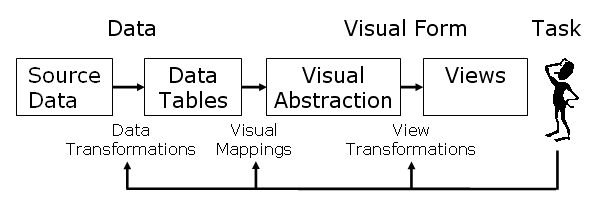
\includegraphics[width=\columnwidth]{figures/reference_model}
\caption{The Information Visualization Reference Model (drawing by
  J. Heer)}
\label{fig:refmodel}
\end{figure}


\subsection{Standardization processes}
ISO, Internet, SQL





